\selectlanguage{british}%

\chapter{Epilogue}


\section{Implications}

In this section, non-contextuality (see \prettyref{sec:Peres-Mermin-Revisited})
will be assumed and notation will be borrowed from \prettyref{sec:Multiplicativity}.
We will use our understanding from multiplicativity, to investigate
it's relationship between entanglement, locality and superposition. 


\subsection{Superposition}

It is known that for simultaneous eigenstates of $\hat{B}_{i}$, multiplicativity
must hold. Consequently, any violation of multiplicativity must arise
from states that are superpositions (of the simultaneous eigenkets).
Note however, that entanglement is not necessary to show a violation,
since the PM test is a state independent test, where a separable state
can be used to arrive at a contradiction. 


\subsection{Non Locality and Entanglement}

It is known from \prettyref{sec:Bell's-Theorem} that $\left\langle \hat{B}\right\rangle \le2$,
where $\hat{B}$ is the Bell operator as defined there. If we assume
(1), (2) and (3), as given in \prettyref{sec:Peres-Mermin-Revisited},
then also it can be proven that $\left\langle \hat{B}\right\rangle \le2$.
To see this, consider $\hat{B}_{1}=\hat{a}_{1}\otimes\hat{\mathbb{I}}$
and $\hat{B}_{2}=\hat{\mathbb{I}}\otimes\hat{b}_{1}$, so that $[\hat{B}_{1},\hat{B}_{2}]=0$
and $\hat{C}\equiv\hat{B}_{1}\hat{B}_{2}$. From multiplicativity,
it follows that $m_{1}(\hat{C})=m_{1}(\hat{B}_{1})m_{1}(\hat{B}_{2})$.
This entails that $m(\hat{a}_{1}\otimes\hat{b}_{1})=m(\hat{a}_{1}\otimes\hat{\mathbb{I}})m(\hat{\mathbb{I}}\otimes\hat{b}_{1})$,
where the subscript has been suppressed for brevity. Note that $m(\hat{*})$,
will depend on the state $\left|\psi\right\rangle $ and the hidden
variables. Therefore, averaging multiple measurements, corresponds
to averaging over the hidden variables. This is expressed by $\left\langle m(\hat{a}_{1}\otimes\hat{b}_{1})\right\rangle =\left\langle m(\hat{a}_{1}\otimes\hat{\mathbb{I}})\right\rangle \left\langle m(\hat{\mathbb{I}}\otimes\hat{b}_{1})\right\rangle $.
One can repeat this argument for each term in $\left\langle \hat{B}\right\rangle $.
Using the fact that $-1\le m(\hat{*})\le1$, and that the extrema
will occur only at the extreme values of $m$, one can plugin $\pm1$
for each $\left\langle m(\hat{*})\right\rangle $ to obtain $\left\langle \hat{B}\right\rangle \le2$.
We can therefore conclude that a violation of Bell's inequality, entails
that atleast one of the three assumptions is wrong. 

One can infact try to show how a consistent (with QM) non-multiplicative
theory, must be non-local. Formally it is clear, since a violation
of Bell's inequality implies non-locality. Consequently, any consistent
completion of QM, will be non-local. More insight can be gained, although
some care is needed. The notion of compatible observables is that
commuting observables don't disturb each other and can be simultaneously
known. While the statement is not precisely stated, we only need to
note that $m_{k_{1}}(\hat{C})=m_{k_{2}}(\hat{B}_{1})m_{k_{3}}(\hat{B}_{2})$,
for $(k_{1},k_{2},k_{3})\in\{(1,2,3),(2,1,3),\dots\}$. In words,
this means that to measure $\hat{C}$, one can instead first measure
$\hat{B}_{1}$ and then measure $\hat{B}_{2}$. A multiplication of
the values obtained, can be taken to be the value a measurement of
$\hat{C}$ yields. This can be verified by measuring $\hat{C}$ subsequently.
The Bell scenario offers an interesting freedom, by restricting the
form of $\hat{B}_{i}$. To evaluate $\left\langle \hat{B}\right\rangle $,
one is required to evaluate $\left\langle \hat{B}_{1}\hat{B}_{2}\right\rangle $.
From the compatibility argument, we need to find the average value
of $m_{3}(\hat{B}_{1}\hat{B}_{2})=m_{1}(\hat{B}_{1})m_{2}(\hat{B}_{2})$,
viz. $\left\langle m_{3}(\hat{a}_{1}\otimes\hat{b}_{1})\right\rangle =\left\langle m_{1}(\hat{a}_{1}\otimes\hat{\mathbb{I}})\right\rangle \left\langle m_{2}(\hat{\mathbb{I}}\otimes\hat{b}_{1})\right\rangle $.
So far, the statements were general. Now we assume that our theory
is non-multiplicative (and non-contextual). A consistent theory (with
QM), using these assumptions, can and must violate $\left\langle \hat{B}\right\rangle \le2$.
However, if the particles are taken far away, then the only way the
theory can be non-multiplicative ($m_{1}(\hat{B}_{1})\neq m_{2}(\hat{B}_{1})$
for example), is if the theory is non-local. Locality will entail
that $m_{1}(\hat{B}_{1})=m_{2}(\hat{B}_{1})$ for instance, since
the information about which observable was measured first, can't be
propagated instantaneously. We see therefore that non-locality arises
quite naturally in consistent non-multiplicative theories.

As a remark, it maybe added that in case of the Bell Test, entanglement
is needed to show one of the three assumptions is wrong. This is so
because it can be shown that entanglement is necessary to arrive at
a violation of the inequality.


\section{Summary of Results}

Progress was made roughly in three categories, as listed. 
\begin{figure}
\begin{centering}
\includegraphics[width=0.75\columnwidth]{Chapter5/Figs/Vector/flow}
\par\end{centering}

\caption{Overview of work done during the semesters. The bold faced titles
represent new results.}
\end{figure}

\begin{itemize}
\item Bohmian Mechanics

\begin{itemize}
\item Generalized the Hamiltonian based measurement scheme to continuous
variables (see \prettyref{sub:BM-measurement-to-continuous})
\item Analytic/graphical proof of consistency check using position measurements
(see \prettyref{sub:BM-Consistency-check-measurement})
\item Analytic/graphical solution to measuring entangled spins using SG
\& using the Hamiltonian scheme (see \prettyref{sub:BM-entangled-Stern-Gerlach},
\prettyref{sub:BM-Hamiltonian-Approach-Spins})
\item Alternative proof of spins can't be associated with particles, and
must only be a property of the wavefunction (see \prettyref{sub:BM-Hamiltonian-Approach-Spins})
\item BM simulator with many trajectories (one particle, one dimensional,
arbitrary potential, see \prettyref{sec:BM-Simulator})
\end{itemize}
\item Tests of Determinism and Contextuality

\begin{itemize}
\item Optimized the phase space GHZ test (see \prettyref{sub:Optimized-Extension})
\item GHZ $\to$ a test of contextuality (see \prettyref{sub:GHZ-to-contextuality})
\item PM extension to phase space (independently re-discovered, see \prettyref{sub:Peres-Mermin-phaseSpace})
\end{itemize}
\item The Contextuality situation

\begin{itemize}
\item BM was shown consistent with PM \& restricted BM was argued to be
non-contextual (see \prettyref{sub:BM-consistent-PM})
\item `Multiplicativity' and `Sequential Multiplicativity' identified, defined
and proven where they hold (see \prettyref{sec:Multiplicativity})
\item Demonstrated `non-multiplicativity' as an alternative to contextuality,
by constructing a toy model (see \prettyref{sub:Non-Contextual-Toy-Model})
\item Proposed the `discretely c-ingle' HV theory to non-contextually explain
spins (see \prettyref{sub:Discretely-C-ingle-Theory})
\end{itemize}
\end{itemize}

\section{Conclusion}

We have shown, that atleast from the Peres Mermin's proof, it doesn't
follow that contextuality is a necessary feature of QM. We have identified
a new property, which we call non-multiplicativity. We have been able
to construct a non-contextual hidden variable theory, that is completely
consistent with QM of spins and it's predictions, we call a discretely
c-ingle theory. This theory is non-multiplicative. 

We also noted that upon restriction of measurement schemes, Bohmian
Mechanics (BM) can also be viewed as a non-contextual hidden variable
theory, which is non-multiplicative. 


\section{Digressions}

As would've been evident so far, the developments made to address
the main problem itself have not always been in the correct direction.
In addition, certain small digressions were made, some of which have
been listed for completeness.


\subsection{Cryptography using contextuality}

Interesting collaborative progress was made in developing certain
cryptography protocols using contextuality, with Jaskaran and Kishor,
who primarily constructed the schemes. A well known idea is to use
entanglement to facilitate secure sharing of keys, where the security
assurance comes from the monogomy of Bell's inequality violations.
An analogue of this idea was used, where the contextuality inequalities
are used in place of Bell's and it was found that the said method
is encouragingly secure and less resource hungry. 


\subsection{Attempt at superluminal communication with BM}

Imagine there are two particles, one with person A, and the other
with person B. Now both measure the position of their particles. Thus
the positions are precisely known. Next, they allow their particles
to evolve under a Hamiltonian (interaction) such that they become
entangled. Suppose at time $t$, the particles are entangled. Now
from the de-Broglie theory, both can predict the locations of their
particles at $t$. Now comes the interesting part. The protocol they
follow, is as follows. Say A uses this setup, only to receive signals.
If B wants to send a signal to A, all that he needs to do, is to disturb
his particle at $t$. This would cause some change in, either the
wavefunction or the position, or both, of the particle, compared to
if B had not caused any disturbance. Now A measures her particle's
position at $t+\epsilon$ and gets the value $q_{A}$. She knows what
position her particle should've been at, if B didn't do anything,
call this position $q_{A}^{(0)}$. If now $q_{A}\neq q_{A}^{(0)}$,
then she knows B sent a signal. If $q_{A}=q_{A}^{(0)}$, then she
knows nothing was sent. Since the equations are non-local, this interaction
is instantaneous, and in principle faster than speed of light.\\
Ofcourse, one can fill in the details, which is what I almost started
doing, but finding the fault in the argument is what was pivotal.
It turns out, the fault was rather straight forward, although a little
subtle. The idea is that regardless of how precise the position measurement
is, its uncertainty will spread with the wavefunction, thereby rendering
any prediction useless. Thus, in this light, chaos restores locality.
This is actually not too hard to see. Imagine you have an uncertainty
$\delta q$, when you measured the position and got the value $q$.
Now we can imagine a gaussian associated with this, as the wavefunction,
after collapse. Since the de-Broglie Bohm theory ensures that the
probability distribution $\left|\psi\right|^{2}$ is preserved by
the dynamics of the particles, as $\psi$ evolves, $\delta q$ will
increase (in case of free evolution), effectively destroying `position
information'. The idea can only be harnessed, if one can somehow decouple
the uncertainty in $q$ from the wavefunction.


\subsection{Identical Particles, an alternate approach}

One difficulty faced when we construct a statistical description of
classical particles, is the Gibbs Paradox. At its heart, is the idea
that one can always distinguish particles, on the basis of their paths.
In QM, identical particles are handled quite elegantly, by (anti-)symmetrization
of the wavefunction. In BM however, the trajectories are again well
known and one might imagine that this signals failure of BM. It so
turns out, that upon appropriately constructing the trajectory space,
invariant under permutations of particles, one is able to stay consistent
with QM and infact, able to gain further insights. 

We realized however, that since QM describes reality, only through
a combination of operators and the state, and that one can take the
view that it is the observer that is incapable of distinguishing which
particle is being looked at, therefore one can imagine that (anti-)symmetrizing
operators should yield effectively the same results as (anti-)symmetrizing
the wavefunctions.

As an illustration, consider the state $\left|\psi\right\rangle =\left|01\right\rangle $.
If this state represented bosons, then we'd have to write according
to the usual methods of QM, $\sqrt{2}\left|\psi_{\text{I}}\right\rangle =\left|01\right\rangle +\left|10\right\rangle $.
Now if we measure say $\hat{\sigma}_{z}\otimes\hat{\mathbb{I}}$,
on $\left|\psi\right\rangle $, we'd obtain $+1$, while the same
measurement on $\left|\psi_{\text{I}}\right\rangle $ would yield
$0$ (on an average, in this case). However, if we instead symmetrize
the operator as $\left(\sigma_{z}\otimes\mathbb{I}+\mathbb{I}\otimes\sigma_{z}\right)/2$,
then even if we measure $\left|\psi\right\rangle $, then on average.
We'd get $0$ upon measuring $\left|\psi_{\text{I }}\right\rangle $
also, as is expected.

I was told by Prof. Mukunda that this has been discussed earlier by
Messiah and Greenberg \cite{symmetrizationIdentical}, in the context
of particle physics. However when considered in view of the Bohmian
formalism, it might yield an interesting alternative to the problem
of identical particles.

\begin{comment}

\section{First Section of the Third Chapter}

And now I begin my third chapter here . . . And now to cite some more
people \cite{prime-number-theorem,texbook,SFPT,latex}


\subsection{First Subsection in the First Section . . .}

and some more


\subsection{Second Subsection in the First Section . . . }

and some more . . . 


\subsubsection{First subsub section in the second subsection . . . }

and some more in the first subsub section otherwise it all looks the
same doesn\textquoteright t it? well we can add some text to it .
. . 


\subsection{Third Subsection in the First Section . . . }

and some more text . . . 


\subsubsection{First subsub section in the third subsection . . . }

and some more in the first subsub section otherwise it all looks the
same doesn\textquoteright t it? well we can add some text to it and
some more and some more and some more and some more


\section{Second section with a Table}

Oh I have a table, which I can to refer (See \ref{tab:My-first-table}).

\begin{table}[H]
\hfill{}%
\begin{tabular}{|c|c|c|}
\hline 
\textbf{1} & \textbf{2} & \textbf{3}\tabularnewline
\hline 
\hline 
4 & 5 & 6\tabularnewline
\hline 
7 & 8 & 9\tabularnewline
\hline 
\end{tabular}\hfill{}

\caption{\label{tab:My-first-table}My first table (I know, it is a really
intuitive name) }
\end{table}
\end{comment}
\selectlanguage{english}%

